%%
% Please see https://bitbucket.org/rivanvx/beamer/wiki/Home for obtaining beamer.
%%
\documentclass[xcolor=dvipsnames]{beamer} 
\usepackage{graphicx}
\usetheme{Frankfurt}
\setbeamertemplate{items}[circle]
\setbeamertemplate{bibliography item}[text]

% Auto creates the dots for each slide in a section
\usepackage{remreset}
\makeatletter
\@removefromreset{subsection}{section}
\makeatother
\setcounter{subsection}{1}

\usepackage{amsmath}
\usepackage{amssymb}
\usepackage{amsfonts} 
\usepackage{mathtools}
\usepackage{graphicx}
\usepackage{bm}
\usepackage{subcaption}
\usepackage{fancyvrb}
\usepackage{subfigure}
\usepackage{graphicx,xcolor}
\usepackage{pifont,mdframed}
\usepackage{tikz}
\usepackage{bm}
\usetikzlibrary{fit,positioning}


\newcommand \etr[0] {
    \text{etr}
}

\newcommand \Etr[1] {
    \text{etr}\left( { #1 } \right)
}

%
% Macros
%
\newcommand \cashort[1] { {\todo[color=yello]{#1 -- Cedric}} }
\newcommand \calong[1]  { { \todo[inline,color=yellow]{#1 -- Cedric} } }
\newcommand \gbshort[1] { {\todo[color=cyan!40]{#1 -- Guillaume}} }
\newcommand \gblong[1]  { { \todo[inline, color=cyan!40]{#1 -- Guillaume} } }
\newcommand \mgshort[1] { {\todo{#1 -- Mark}} }
\newcommand \mglong[1]  { { \todo[inline]{#1 -- Mark} } }
\newcommand \bfshort[1] { {\todo[color=green!40]{#1 -- Bryan}} }
\newcommand \bflong[1]  { { \todo[inline,color=green!40]{#1 -- Bryan} } }


% Adds a plus const to the end of a math expression
\def \pcst{+\text{const}}

% A fancy version for capital R
\def \Rcal{\mathcal{R}}

% A fancy version for r
\def \rcal{\mathbf{r}}

% Loss function / log likelihood as appropriate
\def \L{\mathcal{L}}

% KL divergence [Math Mode]
\newcommand{\kl}[2] {
	\text{KL}\left[#1||#2\right]
}

\newcommand \vecf[1] {
    \text{vec}\left(#1\right)
}

\newcommand \ent[1] {
    \text{H} \left[ #1 \right]
}

\newcommand \mut[2] {
    \text{I} \left[ #1 ; #2 \right]
}

\newcommand \dvi[2] {
    \text{D}_\text{VI} \left[ #1; #2 \right]
}

% Starts an expected value expresses [Math Mode]
\newcommand{\starte}[1] {%
	\mathbb{E}_{#1}\left[
}

% Ends an expected value expression [Math Mode]
\def \ende{\right]}

% Starts an varianc expresses [Math Mode]
\newcommand{\startv}[1] {%
	\mathbb{V}\text{ar}_{#1}\left[
}

% Ends an variance expression [Math Mode]
\def \endv{\right]}

%\newcommand \ex[2] {
%    \bigl\langle #1 \bigr\rangle_{#2}
%}
\newcommand \ex[2] {
    \mathbb{E}_{ { #2 } }\left[ #1 \right]
}
\newcommand \var[2] {
    \mathbb{V}ar_{ { #2 } }\left[ #1 \right]
}

\newcommand \halve[1] {
	\frac{#1}{2}
}

\newcommand \half {
    \halve{1}
}

\newcommand \tr { \text{tr} } 

\newcommand \T { ^\top } 

\newcommand \fixme[1] {
    {\color{red} FIXME: #1}
}

\newcommand \vv[1] { \boldsymbol #1 }

\newcommand{\mbeq}{\overset{!}{=}}

\newcommand \diag[1] { \text{diag} \left( {#1} \right) }
\newcommand \diagonal[1] { \text{diagonal} \left( {#1} \right) }

\newcommand \Ed {{ \vv{\xi}_d}}
\newcommand \Edj {{\xi_{dj}}}
\newcommand \Edk {{\xi_{dk}}}
\newcommand \AEdj {{\Lambda(\xi_{dj})}}
\newcommand \AEdk {{\Lambda(\xi_{dk})}}
\newcommand \AEd  {{ \bm{\Lambda}(\bm{\xi}_d) }}

\newcommand \Axi { { \Lambda_{\xi} } }
\newcommand \bxi { { \vv{b}_{\xi} } }
\newcommand \cxi { { c_{\xi} } }


\newcommand \wdoc      { { \vv{w}_d } }
\newcommand \wdt[0]  { { w_{dt} } }
\newcommand \wdn[0]  { { \vv{w}_{dn} } }
\newcommand \wdnt[0]  { { w_{dnt} } }
\newcommand \wdd[0]   { { \vv w_{d} } }
\newcommand \zd[0]   { { \vv z_{d} } }
\newcommand \zdn[0]  { { \vv{z}_{dn} } }
\newcommand \zdnk[0] { { z_{dnk} } }
\newcommand \zdk[0]  { { z_{dk} } }
\newcommand \thd[0]  { { \vv \theta_d } }
\newcommand \thdk[0] { { \theta_{dk} } }
\newcommand \thdj[0] { { \theta_{dj} } }
\newcommand \epow[1] { { e^{#1} } }
\newcommand \pkt     { { \phi_{kt}  } }
\newcommand \pk      { { \vv \phi_k } }
\newcommand \lmd     { { \vv \lambda_d } }
\newcommand \lmdk    { { \lambda_{dk} } }
\newcommand \xd      { { \vv x_d } }
\newcommand \atxd     { A ^\top \bm x_d}
\newcommand \axd     { A\bm x_d}
\newcommand \tsq      { { \tau^2 } }
\newcommand \ssq      { { \sigma^2 } }
\newcommand \tmsq     { { \tau^{-2} } }
\newcommand \asq      { { \alpha^2 } }
\newcommand \amsq     { { \alpha^{-2} } }
\newcommand \sgsq     { { \sigma^2 } }
\newcommand \xvec     { { \vv{x} } }
\newcommand \omk      { { \bm \omega _k } }
\newcommand \omkt     { { \omega_{kt} } }
\newcommand \oma     { { \Omega_A } }
\newcommand \gdn      { { \vv{\gamma}_{dn} } }
\newcommand \gdnk     { { \gamma_{dnk} } }
\newcommand \gdk      { { \gamma_{dk} } }
\newcommand \isigt   { { \Sigma^{-1}_{\bm \theta} } }




\newcommand \halfSig { \frac{1}{2\sigma^2} }

\newcommand \nor[2]   { \mathcal{N} \left( {#1}, {#2} \right) }
\newcommand \nord[3]   { \mathcal{N}_{#1} \left( {#2}, {#3} \right) }
\newcommand \mnor[3]  { \mathcal{N} \left(#1, #2, #3\right) }
\newcommand \norp[3]  { \mathcal{N} \left(#1; #2, #3\right) }
\newcommand \mnorp[4] { \mathcal{N} \left(#1; #2, #3, #4\right) }
\newcommand \mul[1]   { \mathcal{M} \left( {#1} \right) }
\newcommand \muln[2]  { \mathcal{M} \left( {#1},{#2} \right) }
\newcommand \dir[1]   { \mathcal{D} \left( {#1} \right) }
\newcommand \pois[1]  { \mathcal{P} \left( {#1} \right) }
\newcommand \gp[2]    { \mathcal{GP} \left( {#1}, #2 \right) }
\newcommand \dir[1]   { \mathcal{D} \left( {#1} \right) }
\newcommand \gam[2]   { \mathcal{G} \left( {#1}, {#2} \right) }
\newcommand \beta[1]  { \mathcal{B}eta \left( {#1}, {#2} \right) }

\newcommand \lne[1]  { { \ln \left( 1 + e^{ #1 } \right) } }
\newcommand \Tr[1]   { \tr \left(  {#1}  \right) }

\newcommand \roud  { \vv{\rho}_{d}  }
\newcommand \rodk { \rho_{dk} }

\newcommand \exA[1]  { \ex{#1}{q(A)} }
\newcommand \exV[1]  { \ex{#1}{q(V)} }
\newcommand \exT[1]  { \ex{#1}{q(\Theta)} }
\newcommand \extd[1] { \ex{#1}{q(\thd)} }
\newcommand \exTV[1] { \ex{#1}{q(\Theta)q(V)} }

\newcommand \Real[0]  { { \mathbb{R} } }
\newcommand \VReal[1] { { \mathbb{R}^{#1} } }
\newcommand \MReal[2] { { \mathbb{R}^{#1 \times #2} } }
\newcommand \Nat[0]  { { \mathbb{N} } }
\newcommand \VNat[1] { { \mathbb{N}^{#1} } }
\newcommand \MNat[2] { { \mathbb{N}^{#1 \times #2} } }

\newcommand \inv[1] { {#1}^{-1} }
\newcommand \invb[1] { \inv{\left( #1 \right)} }

\newcommand \cn { \textsuperscript{\texttt{[{\color{blue}Citation Needed}]}} }

\newcommand \const { { \text{c} } }

\providecommand \floor [1] { \left \lfloor #1 \right \rfloor }
\providecommand \ceil [1] { \left \lceil #1 \right \rceil }


\newcommand \vt[2] { { #1^{(#2)} } }

\newcommand \hashtag[1] { { \ttfamily \##1 } }

\newcommand \mvy  { \vv{m}_{\vv{y}} }
\newcommand \sigvy { { S_Y } }

\newcommand \mmy  { M_Y      }
\newcommand \md   { \vv{m}_d }
\newcommand \phin { \vv{\phi}_n }
\newcommand \isigma { { \inv{\Sigma} } }

\newcommand \sigv     { { \Sigma_V } }
\newcommand \isigv     { { \Sigma^{-1}_V } }

\newcommand \sigy { { \Sigma_Y } }
\newcommand \isigy { { \Sigma_{-1}_Y } }


\newcommand \omy  { { \Omega_Y } }
\newcommand \iomy { { \inv{\Omega_Y} } }

\newcommand \siga     { { \Sigma_A } }
\newcommand \isiga     { { \Sigma^{-1}_A } }
\newcommand \diagv { { \diag{\nu_1,\ldots,\nu_P} } }

\newcommand \ma { \vv{m}_a }
\newcommand \my { \vv{m}_y }

\newcommand \VoU { V \otimes U }

%\newcommand \one { \mathbb{1} }
\newcommand \one  {{  \mathds{1} }}

\newcommand \lse { \text{lse} }
%\newcommand \lse[0] { \mathrm{lse} }

\newcommand \Axi { { \Lambda_{\xi} } }
\newcommand \bxi { { \vv{b}_{\xi} } }
\newcommand \cxi { { c_{\xi} } }

% Conditional independence 
\def\ci{\perp\!\!\!\perp} % from Wikipedia



% ------ For the eval section

% Multinomial PDF [Math Mode]
% params: 1 - the variable
%         2 - the value
%         3 - the state indicator (e.g. k for a distro with K values)
%         4 - any additional subscript
\newcommand{\mpdf}[4] {
	\prod_{#3} {#1}_{{#4} {#3}} ^ {#2}
}

% Dirichlet PDF [Math Mode]
% params: 1 - the variable
%         2 - the hyper-parameter
%         3 - the state indicator (e.g. k for a distro with K values)
%         4 - any additional subscript
\newcommand{\dpdf}[4] {
	\frac{1}{B({#2})} \prod_{#3} {#1}_{{#4} {#3}} ^ {({#2}_{#3} - 1)}
}

% To simplify the sampling equations, this is indicates
% that the given value has had datapoint "m" stripped out
%
\newcommand{\lm}[1] {
	#1^{\setminus m}
}

\newcommand \model[0] {
    \mathcal{M}
}

\newcommand \perplexity[1] {
    \mathcal{P} \left( { #1 } \right)
}

\newcommand \WTrain {
    \mathcal{W}^{(t)}
}

\newcommand \WQuery {
    \mathcal{W}^{(q)}
}

\newcommand \oneover[1] {
    \frac{1}{ {#1} }
}

\newcommand \samp[1] {
    { #1 }^{(s)}
}

\newcommand \etd[0] {
    \vv{\eta}_d
}



\author{Bryan Feeney, \\
Supervisor: Dr. Ricardo Silva} 
\title[Multitask Admixture Prediction]{Multi-Task Learning of Component Strengths in Non-Conjugate Admixture Models}
\institute[University College London]{
 University College London
}
\date[July 23, 2015]{July 23, 2015}

\begin{document}

%--- the titlepage frame -------------------------%


\begin{frame}[plain]
  \titlepage
\end{frame}




%--- Research - MTL -------------------------%


\section{Introduction}
\begin{frame}{Outline of the Talk}

\begin{itemize}
    \item<1-> Introduction
    \item<2-> Background
    \only<2> {
        \begin{itemize}
            \item Latent-Variable Models of Textual Corpora
            \item Choice of Priors for Topic Models
            \item Multi-Task Learning
        \end{itemize}
    }
    \item<3-> Model
    \only<3> {
        \begin{itemize}
            \item Model Specification
            \item Variational Inference
            \item Non-Conjugate Variational Inference with Bounds
        \end{itemize}
    }
    \item<4-> Results
    \item<5->Future Work
\end{itemize}


\end{frame}

%--- Admixture Modelling -------------------------%

\section{Background}

\begin{frame}{Latent Variable Models of Text}

\only<1,2> {
    \begin{figure}[t]
    \centering
    \resizebox{6cm}{!}{
        %\documentclass{standalone}
%\usepackage{tikz}
%\usepackage{xcolor}
%\usetikzlibrary{fit,positioning}
%\begin{document}
\begin{tikzpicture}
\coordinate (alpha)   at (0,2);
\node (alpha) at (0,2) [circle, draw, inner sep=1pt, fill, label=above:$\alpha$] { };
\node (theta) at (0,0) [circle, draw, text width = 16pt] {$\text{ }\theta$};

\node (b) at (2,2) [circle, draw, inner sep=1pt, fill, label=above:$\beta$] { };
\node (z) at (2,0) [circle, draw, text width = 16pt] {$z_d$};

\node (psis) at (4,2) [circle, draw] {$\phi_k$};
\node (w) at (4,0) [circle, draw, text width = 16pt, fill=gray!50] {$w_{dn}$};

 
\draw[->] (alpha) -- (theta);
\draw[->] (b.east) -- (psis.west);
 
\draw[->] (theta.east) -- (z.west);
\draw[->] (z.east) -- (w.west);
\draw[->] (psis) -- (w);
 
\draw (1,-.7) rectangle (6.,1);
\draw (3,-.6) rectangle (5,.75);
\draw (3.2,1.4) rectangle (4.8,2.6);
 
\node at (5.5,-.5) {$D$};
\node at (4.8,-.3) {$N$};
\node at (4.5,1.7) {$K$};
  
\end{tikzpicture}
%\end{document}
    }
    \end{figure}
}

\only<1,2,6,7,8>{
Classical Mixture Model of Text - One topic per document
\begin{align*}
\vv{\theta} & \sim \dir{\alpha} & z_d & \sim \muln{\vv{\theta}}{1} & w_{dn} \sim \muln{\vv{\phi}_{z_d}}{1}
\end{align*}
}
\only<1,2> {
    Where each of the component vocabularies is drawn $\vv{\phi}_k \sim \dir{\vv{\beta}}$.
}

\medskip

\only<2>{
However in practice this is not what people actually do...
}

\only<3>{ 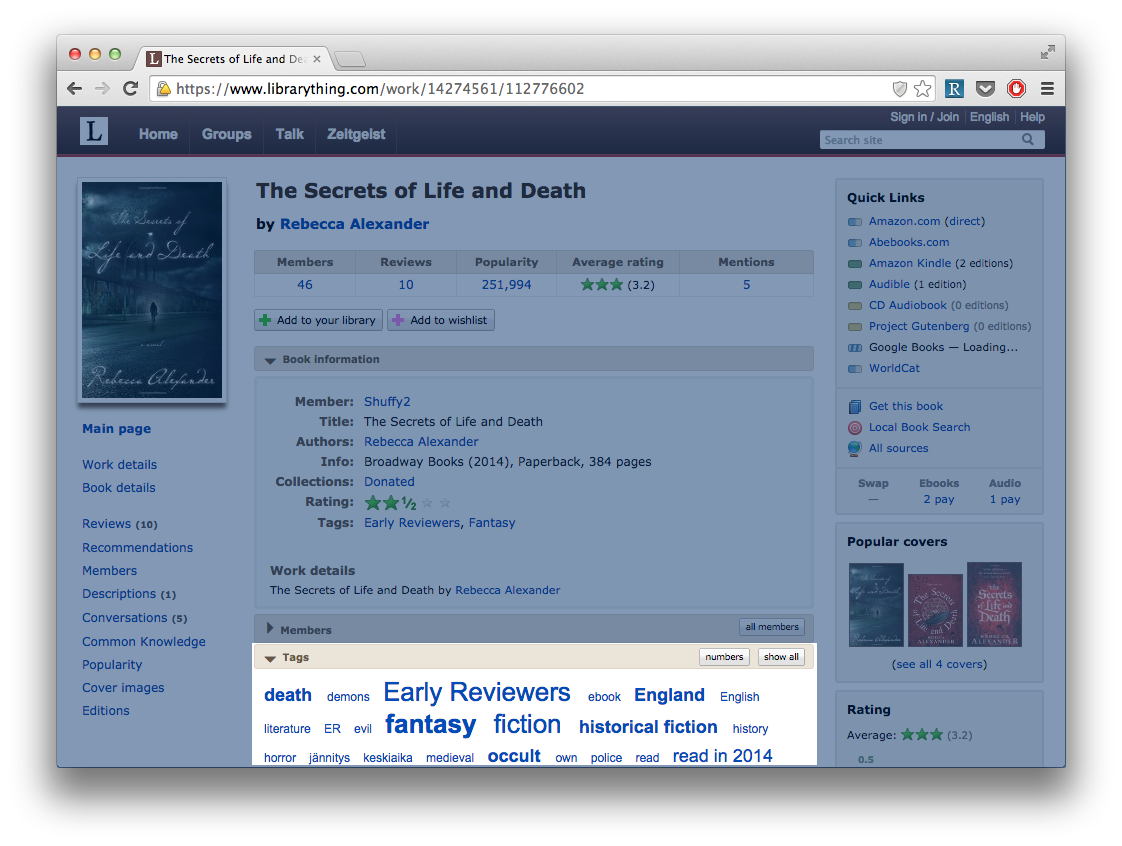
\includegraphics[width=1\textwidth]{images/BookTags.png}}
\only<4>{ 
\includegraphics[width=1\textwidth]{images/NetflixTags.png}}
\only<5>{ 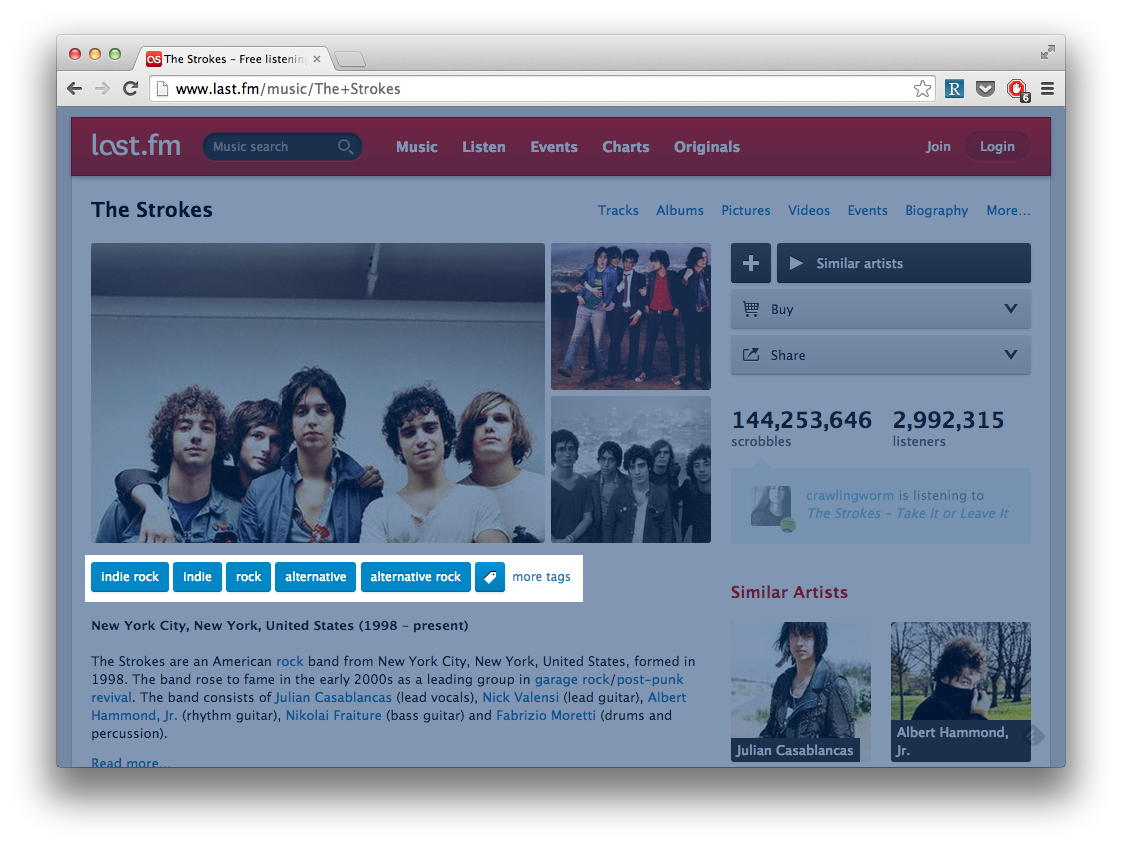
\includegraphics[width=1\textwidth]{images/lastfmTags.png}}

\only<6> {
Mixture models struggle to generalise.
\begin{itemize}
    \item Fewer clusters mean coarser estimates of cluster centroids
    \item But more clusters mean fewer datapoints per cluster, and thus sparser estimates of cluster centroids, due to the assumption of one cluster per document
    \item \fixme{Prediction}
\end{itemize}
}



\only<7,8> {
Admixture models assign a \emph{mixture} of topics to each document\cite{BleiNgJordan2003} 

\begin{align*}
\vv{\theta}_d & \sim \dir{\alpha} & z_{dn} & \sim \muln{\vv{\theta}_d}{1} & w_{dn} \sim \mul{\vv{\phi}_{z_{dn}},1}
\end{align*}

}

\only<7> {
    \begin{figure}[t]
    \centering
    \resizebox{6cm}{!}{
        %\documentclass{standalone}
%\usepackage{amsmath}
%\usepackage{tikz}
%\usepackage{xcolor}
%\usetikzlibrary{fit,positioning}
%\begin{document}

% ---------------------------------------------------
% Comment above for inclusion in other docs
% ---------------------------------------------------


\begin{tikzpicture}
\coordinate (alpha)   at (0,2);
\node (alpha) at (0,2) [circle, draw, inner sep=1pt, fill, label=above:$\alpha$] { };
\node (theta) at (0,0) [circle, draw, text width = 16pt] {$\text{ }\theta_d$};

\node (b) at (2,2) [circle, draw, inner sep=1pt, fill, label=above:$\lambda$] { };
\node (z) at (2,0) [circle, draw, text width = 16pt] {$z_{dn}$};

\node (psis) at (4,2) [circle, draw] {$\beta_k$};
\node (w) at (4,0) [circle, draw, text width = 16pt, fill=gray!50] {$w_{dn}$};

 
\draw[->] (alpha) -- (theta);
\draw[->] (b.east) -- (psis.west);
 
\draw[->] (theta.east) -- (z.west);
\draw[->] (z.east) -- (w.west);
\draw[->] (psis) -- (w);
 
\draw (-0.7,-.7) rectangle (5.5,1);
\draw (1,-.6) rectangle (5,.75);
\draw (3.2,1.4) rectangle (5,2.6);
 
\node at (5.3,-.5) {$D$};
\node at (4.75,-.4) {$N$};
\node at (4.75,1.6) {$K$};
  
\end{tikzpicture}

% ---------------------------------------------------
% Comment below for inclusion in other docs
% ---------------------------------------------------

%\end{document}
    }
    \end{figure}
}

\only<9> {
    Comparing mixture and admixture models for four newsgroups from 20-news.

    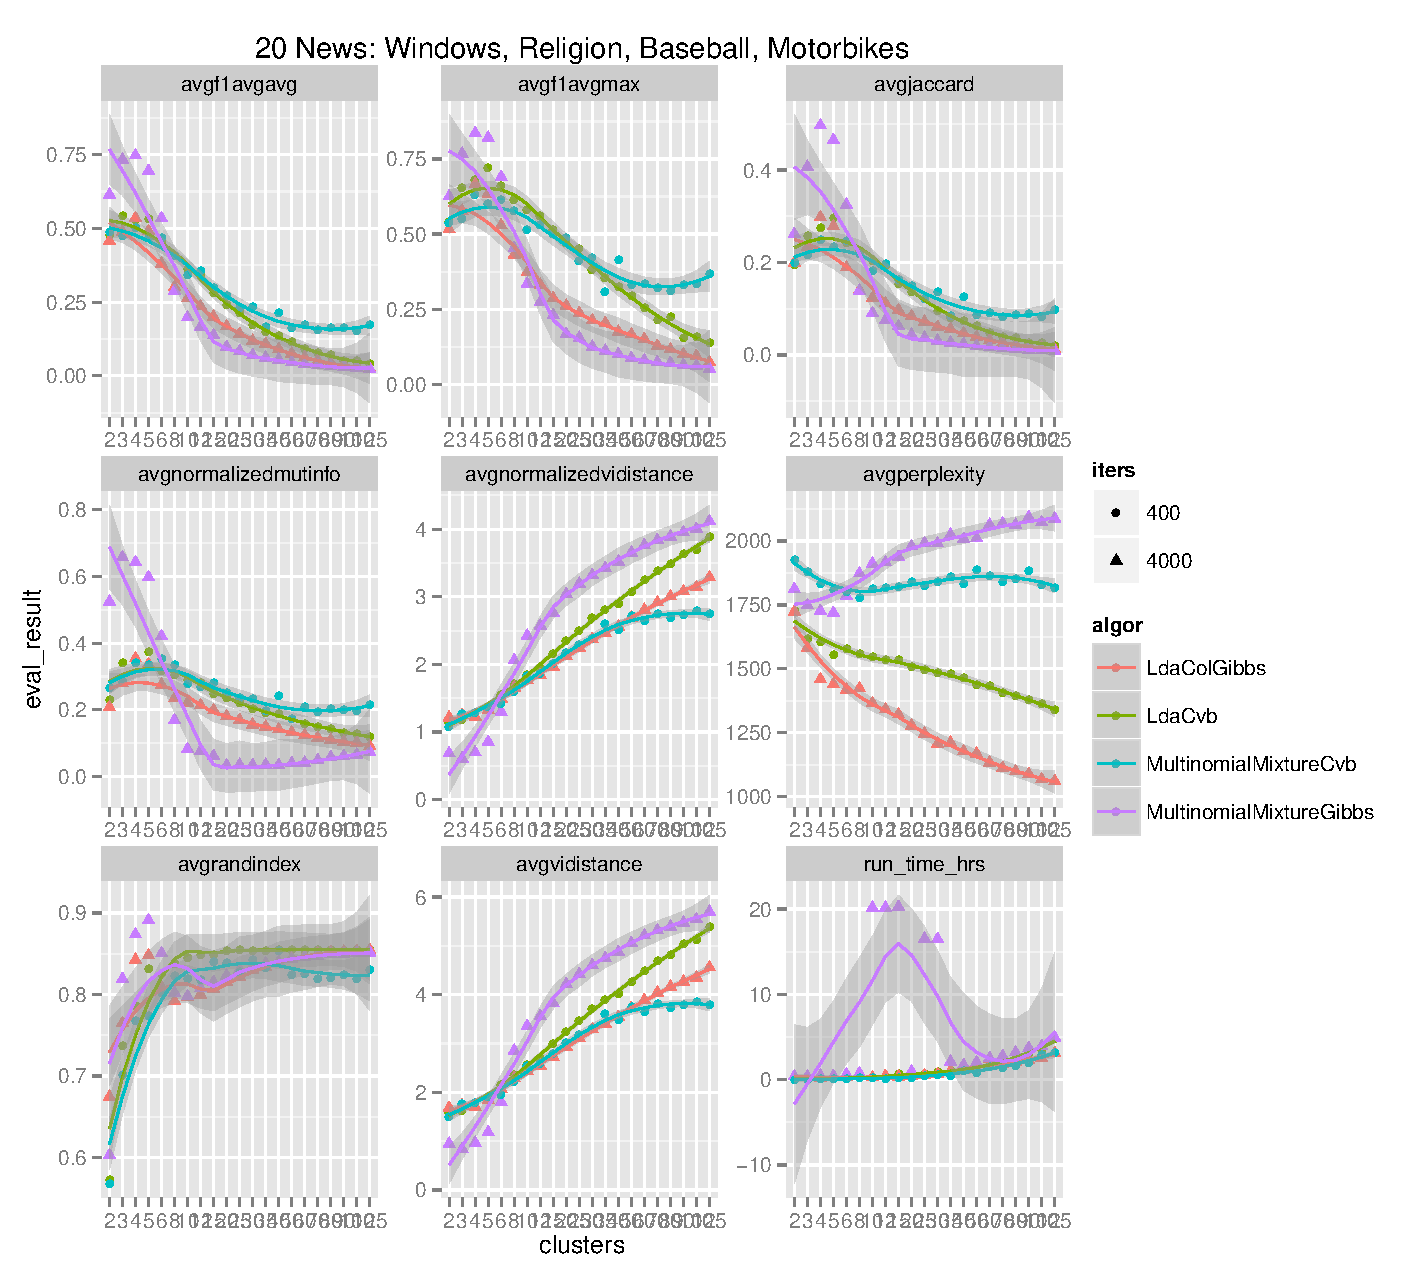
\includegraphics[trim=12.3cm 7.3cm 0.5cm 7.7cm, clip=true, totalwidth=0.8\textwidth]{Images/20news-2013-03-25.pdf}
}


\end{frame}


%--- Topic Model Research -------------------------%


\begin{frame}{Choice of Priors for Topic Models}
\only<1> { 
    The Logistic Normal Distribution
    \begin{itemize}
            \item Captures Correlations between Topics\cite{Blei2006}
        \end{itemize}

        \begin{align*}
        \vv{\theta}_d & \sim \nor{\mu}{\Sigma} & z_{dn} &\sim \muln{\sigma(\vv{\theta}_d)}{1}\\
        & & \sigma(\vv{\theta}_d) & = \frac{\exp(\theta_{dk})}{\sum_j \exp(\theta_{dj})} 
        \end{align*}
    }
    
    \only<2> { 
    The Use of Covariates: $p(\wdoc | \xd) = \int p(\wdoc|\thd) p(\thd|\xd) d\thd$
    \begin{itemize}
        \item Ad-hoc Models: topics over time\cite{Wang2006}, author-topics\cite{MacCallum2007}, regional topics\cite{Eisenstein2010}
        \item Generic approach: Dirichlet Multinomial Regression (DMR)\cite{Mimno2008}.
        \begin{align*}
        \vv{\theta}_d & \sim \dir{\vv{\alpha}_d} & \alpha_{dk} = \exp(\vv{w}_k\top\xd)
        \end{align*}

    \end{itemize} 
    }

\end{frame}


%--- ---- MTL -------------------------%


\begin{frame}{Multi-Task Learning}
Problem: Making many predictions from the same idea
\begin{enumerate}
    \item Predict exam scores in $L$ subjects for several children\cite{Bonilla2008}
    \item Predict customers affinity to $L$ observed aspects of a product\cite{Allenby1999}
    \item Propose image captions by predicting $p(\text{word}|\text{image})$ from image features for every individual word (in this case $L > 10,000$)\cite{Archambeau2011}
\end{enumerate}

\medskip 
\pause

Three general approaches:\cite{Caruana1997}
\begin{enumerate}
    \item Learn correlations between tasks.
    \item Learn structure of features by how we use them - via regularization
    \item Learn a low-rank projection of the tasks themselves
\end{enumerate}
\end{frame}


%--- Regularization -------------------------%



\begin{frame}{Regularization}

\only<1->{
Learn $L$ vectors $\vv{w}_l$. How to \emph{transfer} knowledge from inferring $\vv{w}_1, \ldots, \vv{w}_{l-1}$ to the task of inferring $\vv{w}_l$
}

\medskip 

\only<2>{
    Bayesian approach - learn the prior\cite{Allenby1999}
    
    \begin{align*}
        y_{nl}|\vv{w}_l & \sim \nor{\vv{w}_l\T\vv{x}_n}{\sigma^2 I} & \qquad
        \vv{w}_l & \sim \nor{\vv{m}}{\Sigma} \\
        \vv{m}|\Sigma & \sim \nor{\vv{m}_0}{\oneover{\lambda}\Sigma} & \qquad
        \Sigma & \sim \mathcal{W}^{-1}\left(\Sigma_0, \nu\right)
    \end{align*}
    
    For heterogeneous tasks one can use a mixture model as a prior.
}



\only<3>{
    Low-Rank Projections of the Feature Space  
    \begin{align*}
        y_{nl}|\vv{w}_l & \sim \nor{\vv{w}_l\T\vv{x}_n}{\sigma^2 I} & \qquad
        \vv{w}_l|\vv{z} & \sim \nor{U \vv{z}_l}{\alpha^2 I} \\
        & & \qquad \vv{z}_l & \sim \nor{\vv{0}}{I} \\
        \implies \vv{w}_l & \sim \nor{\vv{0}}{\alpha^2 I + U U\T}  
    \end{align*}
}

\end{frame}


%--- Regularization and Correlation -------------------------%

\begin{frame}{Regularization and Correlation}
Once can also take into account task correlation by setting $W = \left\{ \vv{w}_l \right\}_{l=1}^L$ (note $W \in \MReal{L}{F}$), and defining

\begin{align*}
    \vv{y}_n|W & \sim \nor{W\vv{x}_n}{\Sigma} & \vv{w}_l \sim \nor{0}{\Omega}
\end{align*}

where $\Sigma \in \MReal{L}{L}$ is the \emph{task} covariance, $\Omega \in \MReal{F}{F}$ is the \emph{feature} covariance, and these are learnt in the usual manner.


\end{frame}

%%--- Matrix Variate Prior -------------------------%
%
%\begin{frame}{Matrix-Variate Priors}
%Matrix-Variate Normal Distribution \cite{Gupta1999} :
%\begin{align*}
%W \sim \mnor{M}{\Omega}{\Sigma} & \implies \vecf{W} \sim \nor{\vecf{M}}{\Sigma \otimes \Omega}
%\end{align*}
%
%{ \fontsize{9}{11}\selectfont
%\begin{align*}
%\ln p(W) = -\halve{FL} \ln 2\pi - \halve{F}\ln |\Omega| - \halve{L} \ln | \Sigma | - \half \text{etr} \left( \inv{\Sigma} (W - M) \inv{\Omega} (W - M)\T \right)
%\end{align*}
%}
%where $\text{etr}(X) = \exp \left( \Tr{X} \right)$\\
%
%\bigskip
%\pause
%Matrix Variate Priors for Multi-Task Learning\cite{Bonilla2008}\cite{Archambeau2011}
%, infer $Y \in \MReal{D}{L}$ from $X \in \MReal{D}{F}$
%
%\begin{align*}
%Y | W & \sim \mnor{XW}{I_D}{\Sigma} & \quad W \sim \mnor{0}{\Omega}{\Sigma} \\
%Y &\sim \mnor{0}{I_D + X \Omega X\T}{\Sigma}
%\end{align*}
%Defining a multi-task Gaussian Process regression model\cite{Bonilla2008}.
%
%\end{frame}
%




%--- Research -------------------------%

\section{Model}
\begin{frame}{Motivation}

\begin{itemize}
    \item Predicting component strengths for topic-models with the aid of observed covariates
    \item Use a matrix-variate prior over weights to jointly
    \begin{itemize}
        \item Capture correlations between topics
        \item Capture a low-rank projection of the feature-covariance      
    \end{itemize}
    \item The topic-model itself captures a low-rank representation of word-counts  
\end{itemize}

\pause
Use-Case: Micro-Documents
\begin{itemize}
    \item Tweets: Predict text given user features (username, time tweet was posted). 
    \pause        
    \item In particular predict absent words such as \strong{hashtags}.
\end{itemize}

\end{frame}


%--- Matrix Variate ----------------%

\begin{frame}{Matrix-Variate Normal Distribution}
\begin{align*}
X & \sim \mnor{M}{\Omega}{\Sigma} & \implies \vecf{X} & \sim \nor{\vecf{M}}{\Sigma \otimes \Omega}
\end{align*}

\only<1> {
    {\small
        \begin{align*}
        X & \in \MReal{K}{F} &
        M & \in \MReal{K}{F} &
        \Sigma & \in \MReal{K}{K} &
        \Omega & \in \MReal{F}{F}
        \end{align*}
    }
}

\only<2> {
    {\small
        \begin{align*}
        \ln p(X) = \frac{KD}{2}\ln 2\pi - \frac{K}{2}\ln |\Omega| - \frac{F}{2}\ln |\Sigma| -\half \Tr{\inv{\Sigma}(X - M)\inv{\Omega}(X - M)\T}
        \end{align*}
    }
}

\end{frame}



%--- Model -------------------------%

\begin{frame}{Model}

\only<1> { The Correlated Topic-Model }
\only<2> { Predicting the Mean from Features}
\only<3->{Our Model: Correlation with Low-Rank Feature Covariance}
\only<1> {
    \begin{align*}
    \vv{\theta}_d & \sim \nor{\vv{\mu}}{\Sigma} & z_{dn} & \sim \muln{\sigma(\thd)}{1} \\
    & & w_{dn} & \sim \muln{\vv{\phi}_{z_{dn}}}{1} 
    \end{align*}
}
\only<2> {
    \begin{align*}
    \vv{\theta}_d & \sim \nor{A\xd}{\Sigma} & z_{dn} & \sim \muln{\sigma(\thd)}{1} \\
    & & w_{dn} & \sim \muln{\vv{\phi}_{z_{dn}}}{1} 
    \end{align*}
}

\only<3-> {
    \begin{align*}
    V & \sim \mnor{0}{I}{I} & A|V & \sim \mnor{UV}{I}{\Sigma} \\
    \vv{\theta}_d & \sim \nor{A\xd}{\Sigma} & z_{dn} & \sim \muln{\sigma(\thd)}{1} \\
    & & w_{dn} & \sim \muln{\vv{\phi}_{z_{dn}}}{1} 
    \end{align*}
}

\only<3> {
    \begin{align*}
    A & \sim \mnor{0}{I + UU\T}{\Sigma} 
    \end{align*}
}

\only<4> {
    \begin{itemize}
        \item Learns a low-rank covariance over features $I + UU\T$
        \item Learns correlations between topics, $\Sigma$
        \item Learns a low-rank projection of words via the vocabularies $\vv{\phi}_k$
    \end{itemize}
}

\end{frame}

\begin{frame}{Variational Inference}
\only<1-> {
    Learn a posterior $q(V,A,\Theta,Z,\Phi)$ and parameters $\Sigma, U$. \\
    \medskip
}\only<2> {
    For concave functions $f(x)$ Jensen's inequality states that
    \begin{align*}
    f \left( \ex{X}{q} \right) \geq \ex{f(X)}{q}
    \end{align*}
}
\only<3-> {
    Using Jensen's bound, we derive a bound (the ``free-energy") on the marginal log-likelihood
    \begin{align*}
    \ln p(W,X) \geq \ex{\ln p(W,X,V,A,\Theta,Z,\Phi | \Sigma, U}{q} + \ent{q}
    \end{align*}
}
\only<4-> {
    As the posterior is not tractable, we use the ``mean-field factorization"
    \begin{align*}
    q(V,A,\Theta,Z,\Phi) = q(V)q(A)\prod_d q(\thd)\prod_n q(z_dn) \prod_k q(\vv{phi}_k)
    \end{align*}
}
\only<5-> {
    Most posteriors follow the usual mean-field form, e.g.
    \begin{align*}
    \ln q(A) \propto \ex{\ln p(W,X,V,A,\Theta,Z,\Phi}{q(W,X,V,\Theta,Z,\Phi)}
    \end{align*}
}
\end{frame}


%--- Non-Conjugate Bounds -------------%

\begin{frame}{Non-Conjugate Inference with Quadratic Bounds}
\only<1-> {
    \begin{align*}
    \ln \sigma(\thd) & = \thd - \lse(\thd) & \lse(\thd) = \ln \sum_k \theta_{dk}
    \end{align*}
}

\only<2-> {
    \begin{align*}
    \lse(\vv{y}) & \leq \half \vv{y}\T \Axi \vv{y} - \bxi\T\vv{y} + \cxi
    \end{align*}
}

\only<3-> {
    Bouchard Bound\cite{Bouchard2007}
    \begin{align*}
    \Axi & = \half (I_F - \frac{1}{L} \one \one \T) \\
%    \bxi & = A \vv{\xi} - \sigma(\vv{\xi})\\
%    \cxi & = \half \vv{\xi}\T A \vv{\xi} - \sigma(\vv{\xi})\T\vv{\xi} + \lse(\vv{\xi})
    \end{align*}
}

%\only<4-> {
%    Bohing Bound\cite{Bohning1988a}
%    \begin{align*}
%    \Axi & = \diag{\frac{1}{2\xi_l} \left( \frac{1}{1 + e^{-\xi_l}} - \half\right) }_{l=1}^L  \\
%    \bxi & = \half - 2 s \text{ }\diag{\Axi} \\
%    \cxi & = s - \half (s + \vv{\xi})\T\one + s^2\Axi \one\T\one + \vv{\xi}\Axi\vv{\xi} + \text{vec}_l(\ln (1 + e^{\xi_l}))
%    \end{align*}
%}

\end{frame}



%--- Datasets -------------------------%

\begin{frame}{Model}

Two Datasets
NIPS Papers from 1987 to 1999
\begin{itemize}
    \item 682 Documents. Vocabulary of 12503 words
    \item Median document length of 1,532 words, total of 1,075,323 words across the corpus
    \item Features are: authors; citations; {\color{gray} the year}
\end{itemize}

Tweets from April to September 2013 (inclusive)
\begin{itemize}
    \item 735,868 tweets from 572 users. Vocabulary of 82,698 words
    \item Median tweet length is 10 words (genuinely!), total of 7,272,228 word observations across the corpus 
    \item Features are: authors; time at various granularities (hour, day, week, month)
\end{itemize}

\end{frame}







%--- the Bibliography frame -------------------------%

\section{Reference}
\begin{frame}[allowframebreaks]{Reference}


\bibliographystyle{plain}
\bibliography{/Users/bryanfeeney/Documents/library.bib}


\end{frame}



\end{document}